\appendix
\chapter{Neural Networks}

\label{ch:appendix}

\section{Types of Neural Networks architectures}

            \subsection{Feedforward Neural Network}
            
            \par A Feedforward neural network has the most simple architecture, the data only travels in one single direction. It goes through the input node and exits at the output node. Since there is no back-propagation algorithm this neural network is not able to correct itself \cite{ArmaanMerchant2018} \cite{VikasGupta2017}.

            \begin{figure}[H]
                \centering
                \captionsetup{justification=centering}
                \includegraphics[width=0.5\textwidth]{Sections/2StateOfTheArt/2_images/neural-network.pdf}
                \caption[Feedforward Neural Network]{Example of a Feedforward Neural Network with one hidden layer (with 5 neurons) \cite{neural_image}. }  
            \end{figure}

            \subsection{Radial Basis Function Neural Network}

            \par This network is composed of two layers. In the first one features are combined with a radial basis function in the inner layer. The second one is the output, where these features are taken in consideration while computing the same output in the next function.
            \par A radial basis function means that the distance of a point is considered with respect to the center \cite{ArmaanMerchant2018}.


            \subsection{Recurrent Neural Network (RNN)} 

            \par Recurrent Neural Networks (RNNs) are designed to recognize sequential data characteristics and use patterns to predict the next likely scenario. In these kind of neural networks the signals are propagated in both directions as well as within the layers. They work on the principle of saving the output of a layer and feeding it to the input to help in the prediction of the outcome of the layer.
            \par RNNs use the back-propagation algorithm which allows to make sure that the output is correct almost 100\% of the time \cite{ArmaanMerchant2018}.
        


            \subsection{Convolutional Neural Network (CNN)}
            
            \par CNNs, also known as ConvNets, are a class of deep neural networks that employ the mathematically convolutional operation in at least one of its layers and have a deep feed-forward (not recurrent) architecture \cite{Ribeiro}. They share similarities with feedforward neural networks, since neurons also have weights and biases that are able to learn. In this network the input features are taken like a filter, which allows the network to have memory, since it can remember the images in parts and compute operations like conversion of the image from RGB or HSI to grayscale, allowing the detection of edges and images that can be classified into different categories \cite{ArmaanMerchant2018}. 

            \par The only notable difference between CNNs and traditional ANNs is that CNNs are primarily used in the field of pattern recognition within images. This allows the encoding image-specific features into the architecture, making the network more suited for image-focused tasks, while further reducing the parameters required to set up the model \cite{OShea2015}.
            
            

            \par CNN convolves learned features with input data, and uses 2D convolutional layers which make this architecture one of the best to process 2D data, such as images. They also remove the necessity of manual feature extraction. There is no need to identify features used to classify images since CNNs work by extracting them directly from images. This is important because relevant features are not pretrained, they are learned while the network trains on a dataset \cite{mathworks_deeplearning}.

            \vspace{+2.5cm}
            \begin{figure}[H]
                \centering
                \captionsetup{justification=centering}
                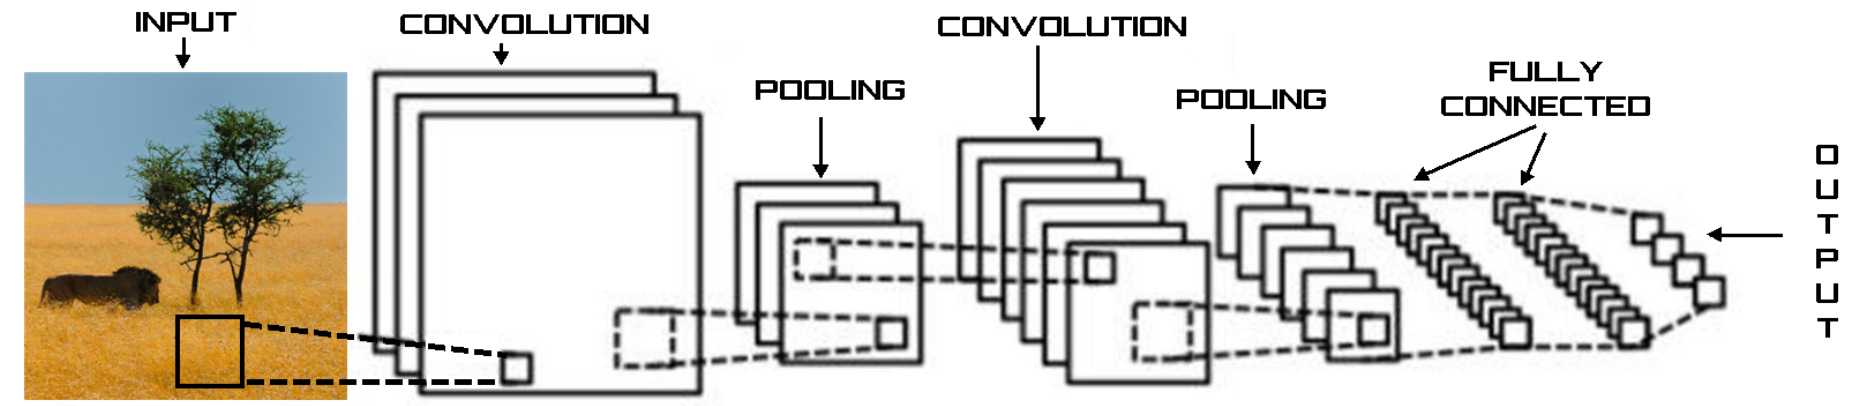
\includegraphics[width=\textwidth]{Sections/2StateOfTheArt/2_images/conv.png}
                \caption[CNN architecture]{CNN architecture \cite{Ribeiro}.}  
            \end{figure}

            \newpage
           \par \textbf{Input Layers}
           \par The input layer is the first layer of a CNN and serves the purpose of resizing an image in order for it  to pass onto further layers for feature extraction \cite{Ribeiro}. It also holds the pixel value of the images \cite{OShea2015}. \bigbreak
            
          
           \par \textbf{Convolutional Layers}
           \par The convolutional layers extracts low-level features from an image, such as edges, color or gradient orientation, according to the applied filter or kernel \cite{Ribeiro}. \bigbreak

           \par \textbf{Activation Functions}
           \par The activation function introduces nonlinearity in order for CNNs to learn functionalities. They serve as decision functions and help in learning complex patterns. Some examples of activation functions are sigmoid, softmax and ReLU \cite{Ribeiro}. \bigbreak

           \par \textbf{Pooling Layers} 
           \par The pooling layers serve the purpose of reducing the parameters required and computation in the network by controlling the overfitting. This is achieved by reducing the spatial size of the network \cite{Ribeiro}.
           \par Overfitting happens when a model learns the detail and noise in the training data to an extent that it negatively impacts the performance of the model on new data \cite{OShea2015}. \bigbreak


           \par \textbf{Fully Connected Layers}
            \par  The final layer in a CNN is usually a fully connect layer used for classification purposes. They take all features from the previous layer and compute class probabilities or scores. These features are then translated into a different class \cite{Ribeiro}.\bigbreak
            
            
%%%%%%%%%%%%%%%%%%%%%%%%%%%%%%%%%%%%%%%%%%%%%%%%%%%%%%%%%%%%%%%%%%%%%%%%%
\section{CNNs architectures For Image Classification}
\label{sec:cnn}
    \subsection{SquezeeNet}
    \label{SquezeeeNet}

    SquezeeNet is a deep neural network for computer vision that is more efficient for distributed training, since it requires less parameters to be transferred. The main goal of SquezeeNet creation was to obtain a smaller neural network with fewer parameters that could more easily fit into a computer memory, making it more easily transmitted over a computer network. This neural network was firstly implemented on top of the caffe deep learning software framework and later ported to the chainer deep learning software framework and Apache MXNET framework.\par
    The basis of SquezeeNet consists in 3 ideas \cite{Iandola2016}:

    \begin{itemize}
        \item Replacing 3x3 filters with 1x1 filters and reduce the number of input channels. This improves computation speed and alleviates the computer resources required, since 1x1 filters have 9 times less parameters than 3x3 filters.
        \item Utilize 1x1 filters as a bottleneck layer to help reducing the computation required for the following 3x3 filters.
        \item Keeping a big feature map by down sampling late.
    \end{itemize}

    

    This neural network is built with fire modules, which are represented in Figure \ref{fig:firemodule}. 


    \begin{figure}[H]
        \centering
        \captionsetup{justification=centering}
        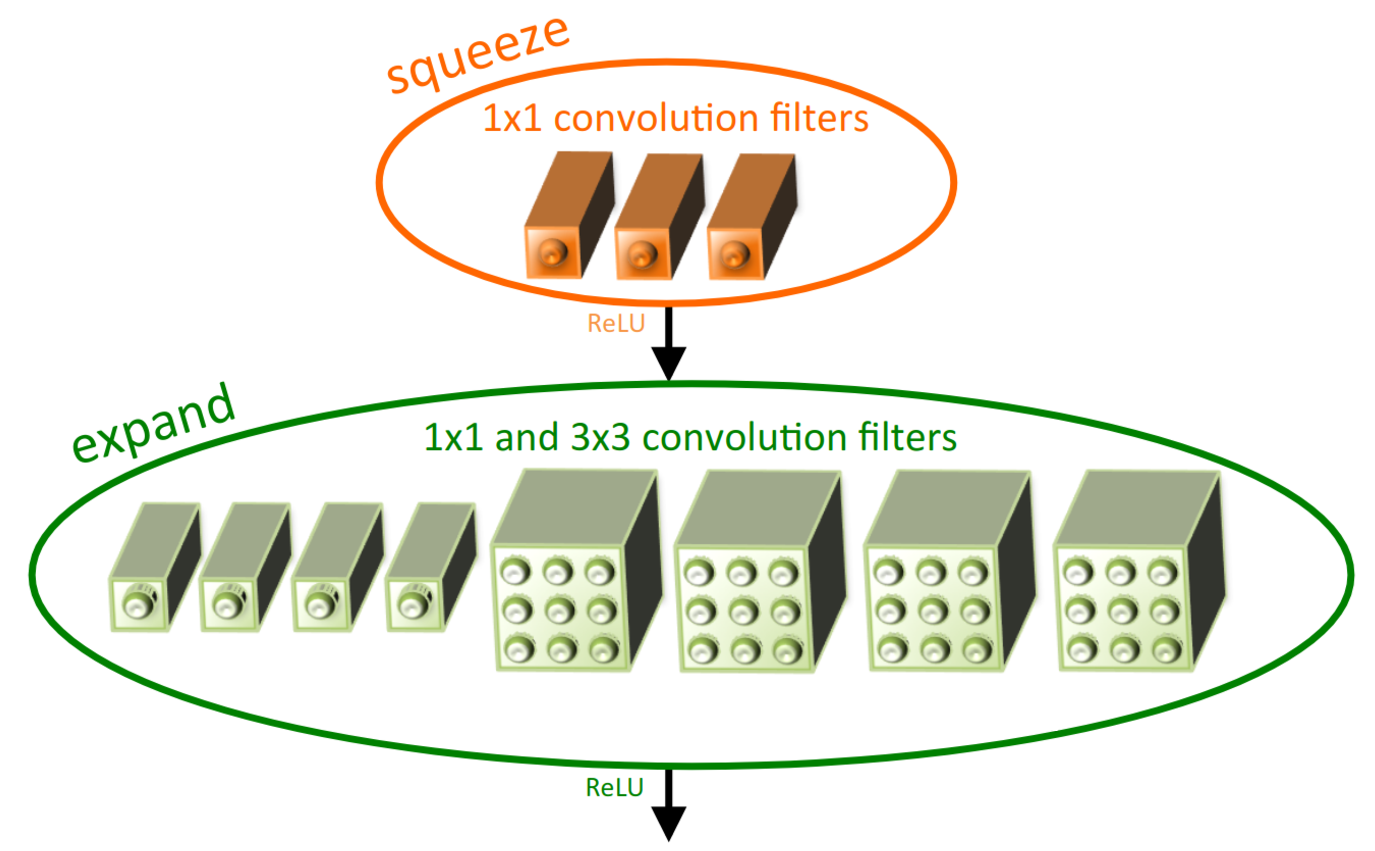
\includegraphics[width=0.6\textwidth]{Sections/2StateOfTheArt/2_images/firemodule.png}
        \caption[SqueezeNet fire module]{SqueezeNet fire module \cite{Iandola2016}.}  
        \label{fig:firemodule}
    \end{figure}
    
    The fire module contains both a squeeze layer and an expand layer. SquezeeNet stacks fire modules and pooling layers  (this can be seen in Figure \ref{fig:squezeenet}). The squeeze layer and expand layer maintain the same feature map size, while the pooling layers reduce the depth to a smaller number, later increasing it. Reducing the depth means the expand layer has fewer computations to do, boosting the speed.\par


    \hfill
    
   \textbf{Squeeze layer architecture: } Consists on 1x1 convolutions, it essentially combines all the channels of the input data into one (and thus reducing the number of input channels needed in the next layer).\par
   \hfill

   \textbf{Expand layer architecture:} Consists on 1x1 convolutions mixed alongside 3x3 convolutions. The 1x1 convolutions combine the channels of the previous layers in various ways. The 3x3 convolutions detect structures in the image since 1x1 convolutions can’t. \par
   \hfill

   \textbf{SquezeeNet architecture:} SquezeeNet doesn’t fully connect layers and it consists of 8 fire modules and a single convolution's layer as input and output. It uses Global Average Pooling, taking each channel from the previous convolution layer and builds an average over all values.



   \begin{figure}[H]
    \centering
    \captionsetup{justification=centering}
    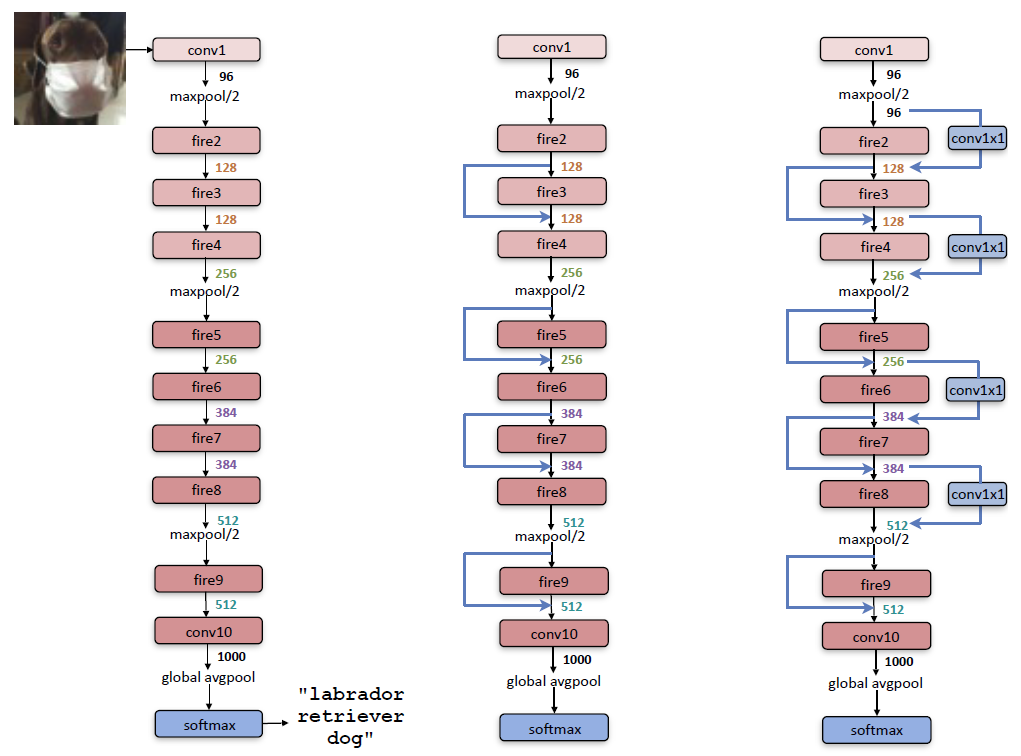
\includegraphics[width=0.75\textwidth]{Sections/2StateOfTheArt/2_images/squezeeNetArchitecture.png}
    \caption[SqueezeNet architecture.]{SqueezeNet architecture. \cite{squeezenetweb}} 
    \label{fig:squezeenet}
\end{figure}


  
    
%%%%%%%%%%%%%%%%%%%%%%%%%%%%%%%%%%%%%%%%%%%%%%%%%%%%%%%%%%%%%%%%%%%%%%%%%%%%%

    \subsection{ResNet}

    The core idea of ResNet (Residual Neural Network) is introducing skip connections (also called identity shortcut connection, represented in Figure \ref{fig:skip}). The way this works is by adding the output of an earlier layer to a later layer in order to jump over some layers. \par

    The vanishing of gradients problem makes deep neural networks hard to train, this happens because as the gradient is propagated back to earlier layers, repeated multiplications may turn the gradient too small, this results in a rapidly performance degradation. Skipping over layers helps avoiding the vanishing of gradients problem and improves the accuracy of the neural network. Having the skip connection allows the training of extremely deep neural networks, more than 150 layers, successfully and still being able to achieve a compelling performance \cite{He2016}.

    This architecture is represented in Figure \ref{fig:resnet}.
    \begin{figure}[H]
        \centering
        \captionsetup{justification=centering}
        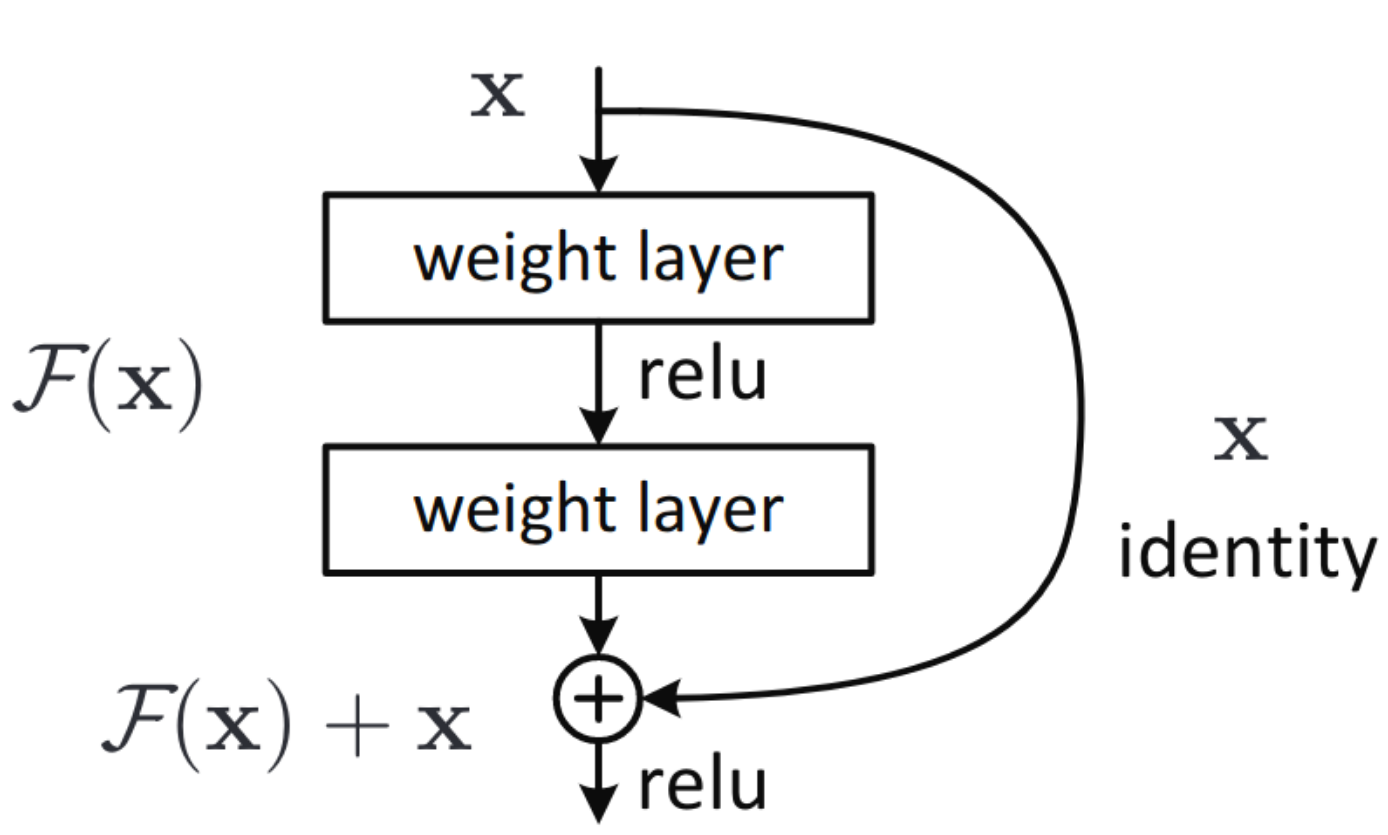
\includegraphics[width=0.4\textwidth]{Sections/2StateOfTheArt/2_images/resnet_block.png}
        \caption[Skipping connection example]{Skipping connection example \cite{He2016}.} 
        \label{fig:skip}
    \end{figure}

    

    \begin{figure}[H]
        \centering
        \captionsetup{justification=centering}
        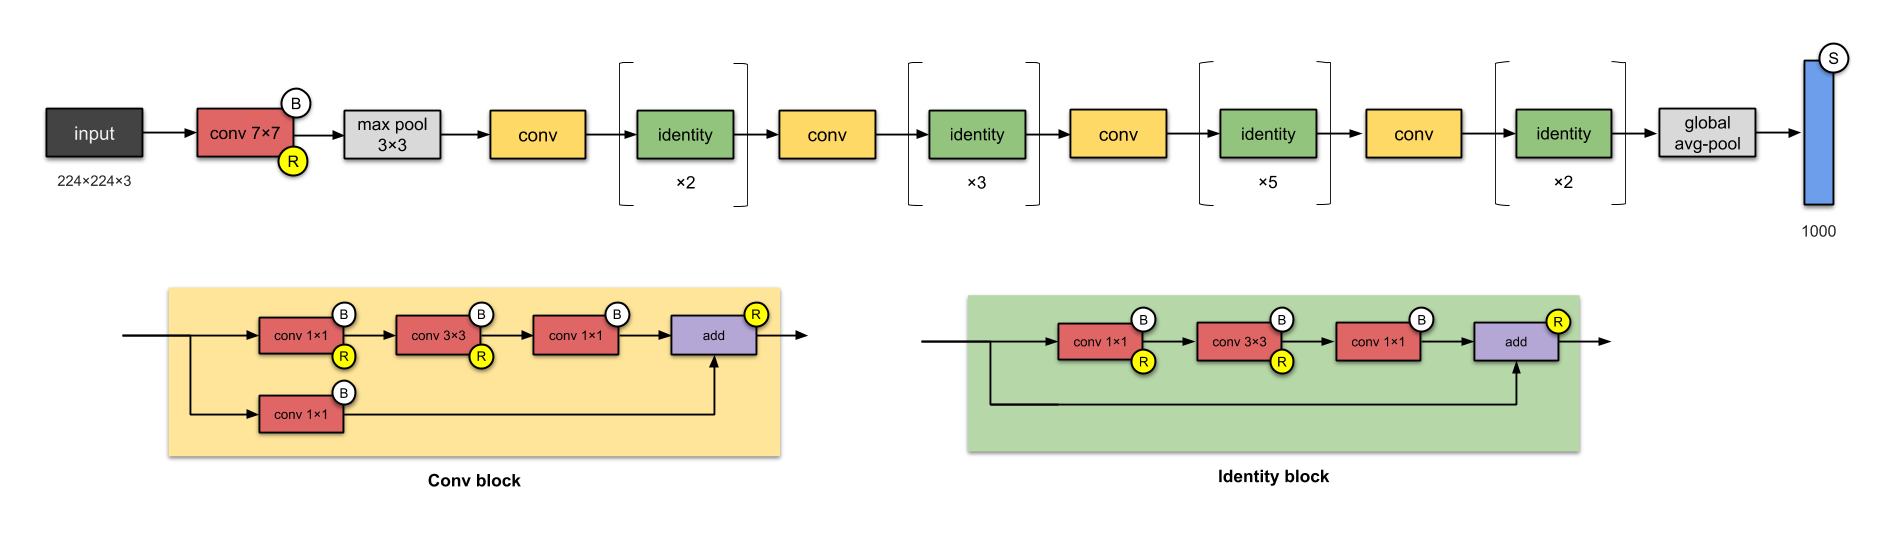
\includegraphics[width=0.85\textwidth]{Sections/2StateOfTheArt/2_images/resnet_arch.png}
        \caption[ResNet architecture]{ResNet architecture \cite{cnnarchitectures}.} 
        \label{fig:resnet}
    \end{figure}

%%%%%%%%%%%%%%%%%%%%%%%%%%%%%%%%%%%%%%%%%%%%%%%%%%%%%%%%%%%%%%%%%%%%%%%%%%%%%

    \subsection{InceptionV3}

    \par Initially named GoogLeNet, the Inception-v1 architecture was proposed by researchers of Google company and was the winner of the ILSVRC 2014 competition, making it historically significant in Convolutional Neural Networks. 
    \par This network, trained on the imageNet dataset, introduced inception modules (shown in Figure \ref{fig:inception_module}) that allowed for a more efficient computation and deeper network.

    \begin{figure}[H]
        \centering
        \captionsetup{justification=centering}
        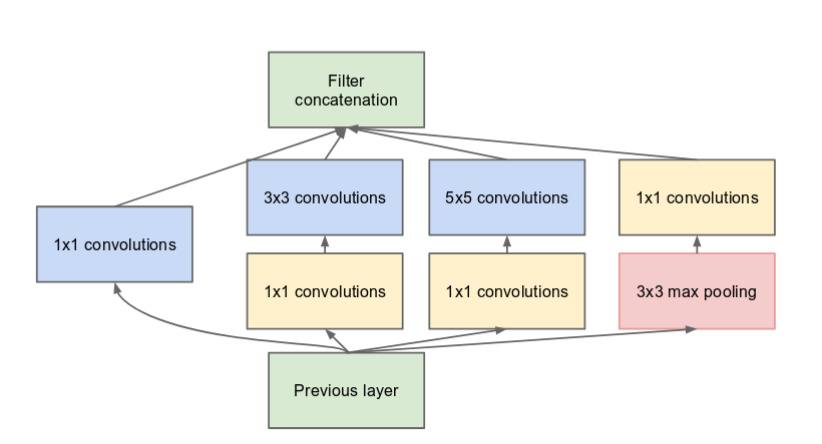
\includegraphics[width=0.5\textwidth]{Sections/2StateOfTheArt/2_images/inceptionArchitecture.png}
        \caption[Inception module]{Inception module \cite{inceptionV3web2}.} 
        \label{fig:inception_module}
    \end{figure}

    \par The Inception architecture (Inception-v1) was improved by the introduction of batch normalization (Inception-v2) \cite{Ribeiro}.


    InceptionV3, is 48 layers deep and able to classify images into 1000 different categories. The improvement over its predecessors is the adding of factorization ideas (Figure \ref{fig:factorization} shows an example of this). 

    \begin{figure}[H]
        \centering
        \captionsetup{justification=centering}
        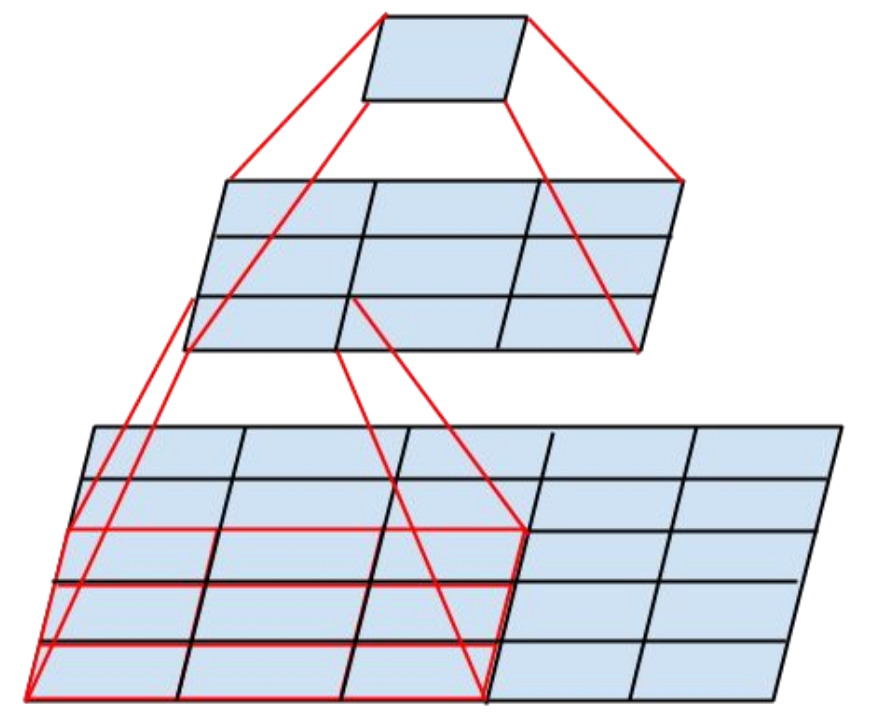
\includegraphics[width=0.35\textwidth]{Sections/2StateOfTheArt/2_images/factor_inception.png}
        \caption[Example of factorization.]{Mini-network replacing the 5×5 convolutions (Example of factorization) \cite{Szegedy2016}.} 
        \label{fig:factorization}
    \end{figure}


    \par This third interaction aims at factorizing convolutions, reducing the number of connections/parameters required while maintaining network efficiency. As an example, using a layer of 5x5 filter requires 5x5=25 parameters, this layer can be replaced by two 3x3 layers which reduce the number of parameters required by 28\%, since 2x(3x3) = 18 parameters. Reducing the number of parameters required reduces the computational resources required and also prevents overfitting. This enables the network to go deeper \cite{inceptionV3web}.
    \par The inceptionv3 architecture can be seen in the figure below.
  
    \begin{figure}[H]
        \centering
        \captionsetup{justification=centering}
        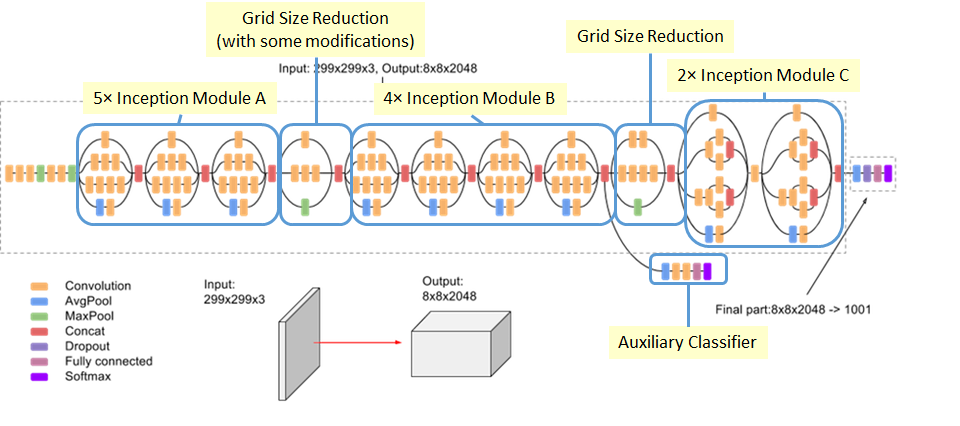
\includegraphics[width=\textwidth]{Sections/2StateOfTheArt/2_images/inceptionv3_architecture.png}
        \caption[InceptionV3 architecture]{InceptionV3 architecture \cite{inceptionV3web}.} 
    \end{figure}

    \par Even though InceptionV4 \cite{szegedy2016inceptionv4} is already available it was not used in this work. The improvements over its predecessor are as follow: 
    \begin{enumerate}
        \item Converting Inception modules to Residual Inception blocks.
        \item Adding more Inception modules.
        \item Adding a new type of Inception module (Inception-A) after the Stem module.
    \end{enumerate}
    
    
    
   

    \newpage
%%%%%%%%%%%%%%%%%%%%%%%%%%%%%%%%%%%%%%%%%%%%%%%%%%%%%%%%%%%%%%%%%%%%%%%%%%%%%
    \subsection{DenseNet}

    Densely Connected Convolutional Networks aim at expanding the depth of deep convolutional networks by connecting each layer to every other layer, in a feed forward fashion (which can be seen in Figure \ref{fig:densenet}), this reduces  the number of parameters required and alleviates the problem of the vanishing-gradients, while improving feature propagation (ensuring maximum information and gradient flow) and feature reuse which allows the learning of more compact and accurate models. This kind of neural network simplifies the connectivity pattern between layers introduced in other architectures (such as ResNets) \cite{Szegedy2016}. \par

    The improved flow of information and gradients makes DenseNets easier to train, since each layer has direct access to the gradients from the loss function and the original input signal, leading to an implicit deep supervision. \par

    DenseNets scale naturally to hundreds of layers, while exhibiting no optimization difficulties.


    \begin{figure}[H]
        \centering
        \captionsetup{justification=centering}
        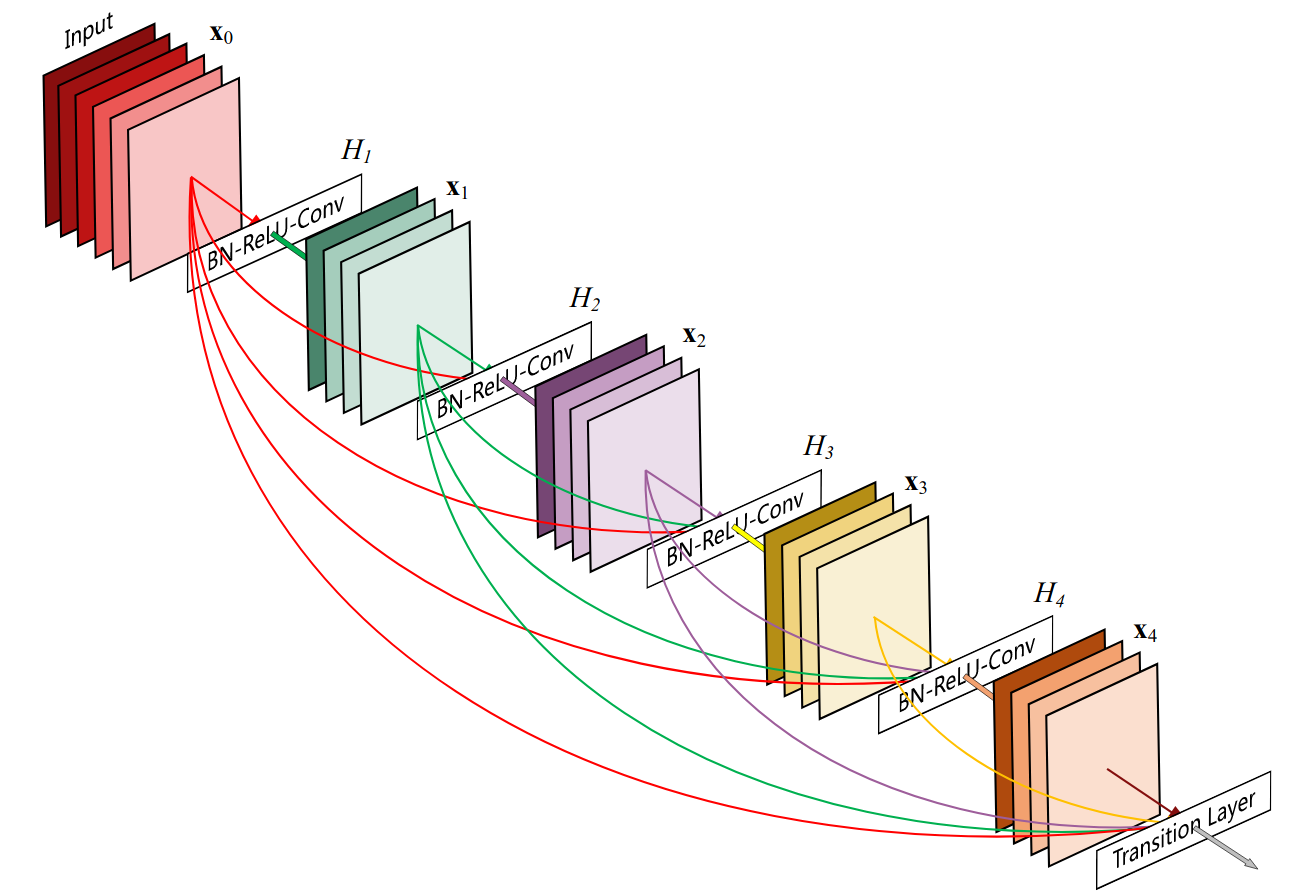
\includegraphics[width=0.45\textwidth]{Sections/2StateOfTheArt/2_images/denseNet.png}
        \caption[DenseNet layers.]{A 5-layer dense block. Each layer takes all preceding feature-maps as input \cite{Szegedy2016}. } 
        \label{fig:densenet}
    \end{figure}
    

%%%%%%%%%%%%%%%%%%%%%%%%%%%%%%%%%%%%%%%%%%%%%%%%%%%%%%%%%%%%%%%%%%%%%%%%%%%%%


\section{Regression based algorithms for Object Detection}
\label{sec:regression}
\par Regression based algorithms (also called single stage detectors) work differently than classification based algorithms. Instead of selecting multiple interesting parts of an image, they predict classes and bounding boxes for the entire image in one single run of the algorithm.
\par These algorithms are extremely fast but are not so accurate as classification based algorithms \cite{Lin2017}. 
RetinaNet, YOLO and SSD are a few examples of object detection algorithms of this type. \par


%%%%%%%%%%%%%%%%%%%%%%%%%%%%%%%%%%%%%%%%%%%%%%%%%%%%%%%%%%%%%%%%%%%%%%%%%%%%%
    \subsection{RetinaNet}

    RetinaNet is a one-stage object detector presented at the 2017 International Conference on Computer Vision by the Facebook AI Research.\par

    In order to improve performance a loss function was implemented, called Focal Loss, allowing the network to focus more on difficult samples. With the loss function, alongside a one-stage network architecture, RetinaNet is able to achieve state-of-the-art performance in terms of accuracy and running time.\par

    This neural network is essential composed of one backbone network and two subnetworks. The backbone network is called Feature Pyramid Net \cite{lin2016feature}, built on top of ResNet, and has the purpose of computing convolutional feature maps of an image. Both subnetworks serve different purposes, one is for object classification using the backbone network output and the other subnetwork is responsible for performing the bounding box regression using the backbone network output \cite{Lin2017}. \par

    In Figure \ref{fig:retinanet} its observable the Feature Pyramid Network (FPN) on top of the convolutional neural network ResNet as a backbone network (a) to generate a rich convolutional feature pyramid (b). The class subnet (c) is for classifying anchor boxes, and the box subnet (d) is for regressing from anchor boxes to ground-truth object boxes. \par 


   
    \begin{figure}[H]
        \centering
        \captionsetup{justification=centering}
        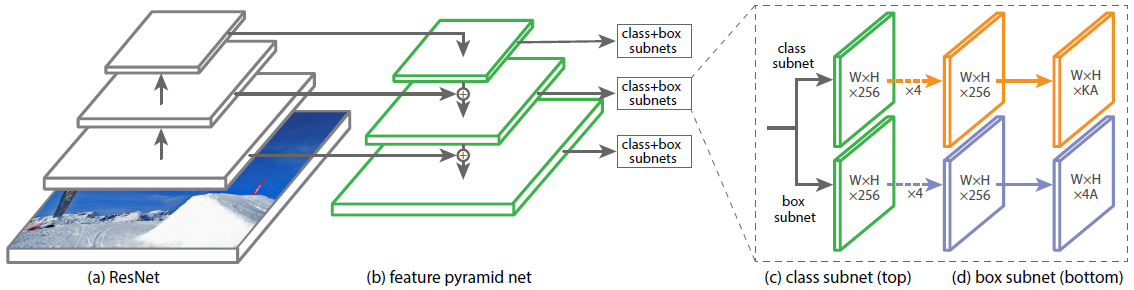
\includegraphics[width=0.85\textwidth]{Sections/2StateOfTheArt/2_images/RetinaNet.png}
        \caption[RetinaNet architecture]{RetinaNet architecture \cite{Lin2017}.} 
        \label{fig:retinanet}
    \end{figure}

%%%%%%%%%%%%%%%%%%%%%%%%%%%%%%%%%%%%%%%%%%%%%%%%%%%%%%%%%%%%%%%%%%%%%%%%%%%%%

    \subsection{YOLOv3}

    YOLOv3 (You Only Look Once version 3) is a state-of-the-art, real-time object detection that’s in the third iteration of the original YOLO, it’s extremely fast and accurate (on par with the accuracy of focal loss from RetinaNet, but 4 times faster). YOLO allows the user to tradeoff between speed and accuracy simply by changing the size of the model.\par

    Compared to other classification networks that perform predictions multiple times for various regions in an image, YOLO architecture is more like a fully convolutional neural network do to the fact that it takes an image as input and passes it only once through the FCNN. The network divides the image into regions and predicts bounding boxes (weighted by predicted probabilities) and probabilities to each region, outputting a vector of bounding boxes and classes predictions. \par 
    
    \par YOLO works by dividing an image in an SxS grid and assuming B bounding boxes per grid. Each of the bounding box predicts 4 coordinates, object and class probabilities \cite{Agarwal2019}.

    \begin{figure}[H]
        \centering
        \captionsetup{justification=centering}
        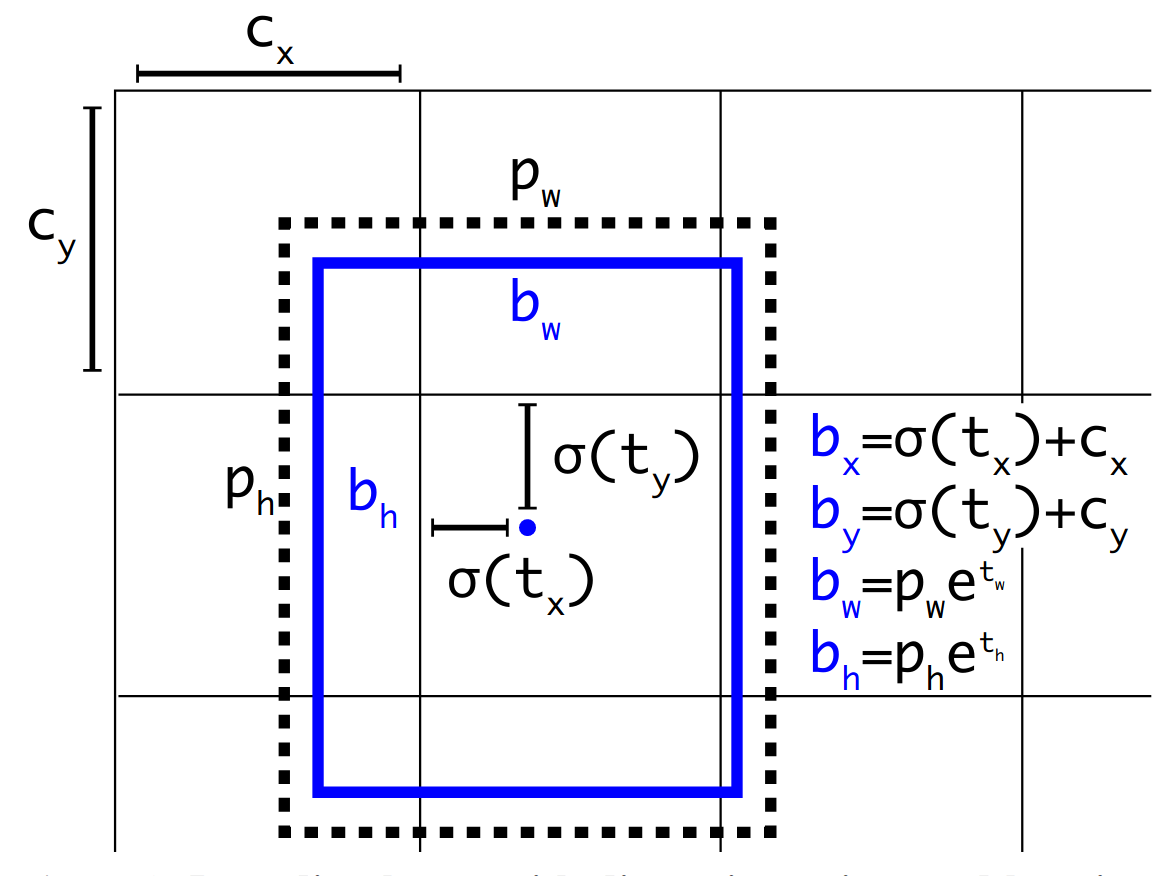
\includegraphics[width=0.4\textwidth]{Sections/2StateOfTheArt/2_images/yolo_boundingbox.png}
        \caption[YOLOv3 bounding box prediction]{Bounding box prediction: predicted box (blue), prior box (black dotted) \cite{Redmon2018}.} 
    \end{figure}

    \newpage
    \par YOLO image predictions are informed by global context in the image since it can look at the entire image at the test time. This gives it several advantages over classifier-based systems. In addition, this algorithm also uses an open source neural network called Darknet-53 for feature extraction, this neural network is written in C and CUDA and it supports CPU and GPU computation \cite{Redmon2018}.\par 
    \par The full architecture of YOLOv3 is represented in Figure \ref{fig:yolov3}.

    \begin{figure}[H]
        \centering
        \captionsetup{justification=centering}
        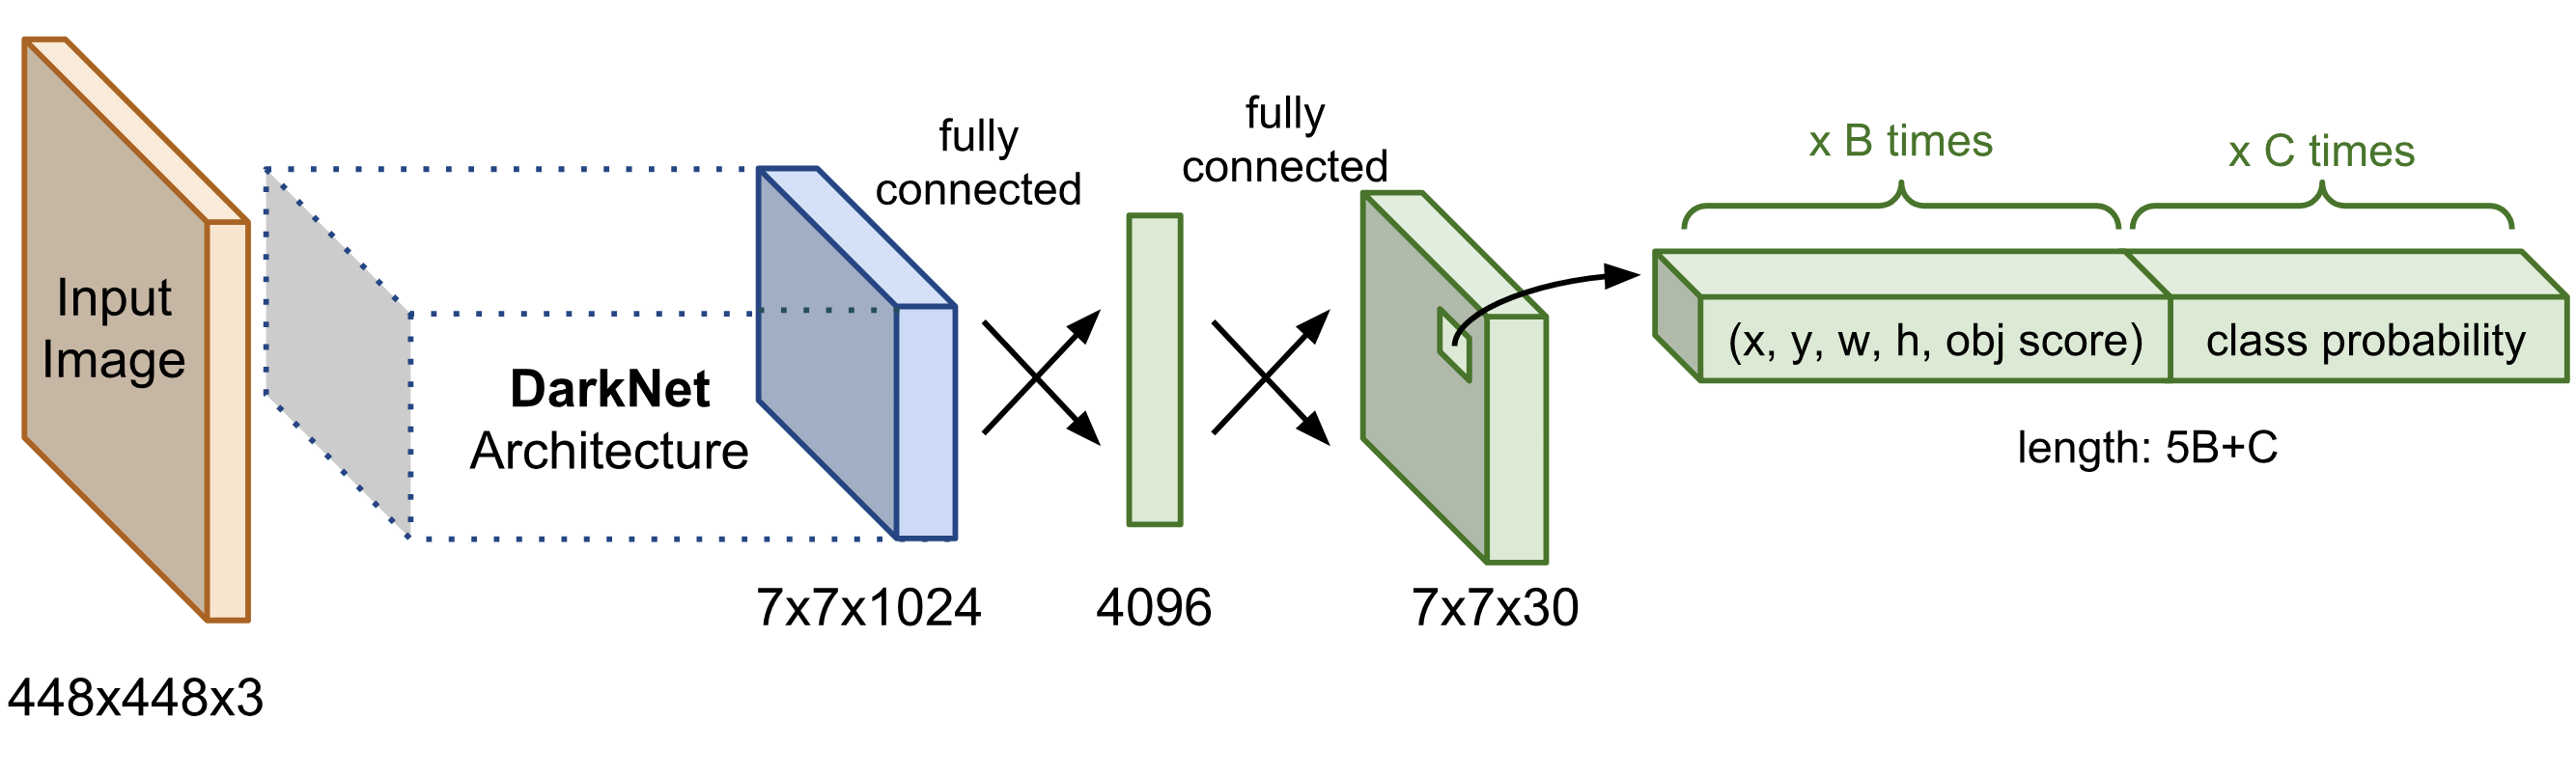
\includegraphics[width=0.85\textwidth]{Sections/2StateOfTheArt/2_images/yolo-network-architecture.png}
        \caption[YOLO base model network architecture.]{The network architecture of YOLO base model \cite{weng2018detection4}.}
        \label{fig:yolov3} 
    \end{figure}

    

   

%%%%%%%%%%%%%%%%%%%%%%%%%%%%%%%%%%%%%%%%%%%%%%%%%%%%%%%%%%%%%%%%%%%%%%%%%%%%%%%

    \subsection{TinyYoloV3}
    \label{sec:tiny_yolo}

    TinyYOLOv3 is a smaller model of YOLOv3 that requires less computational resources since it doesn’t occupy a large amount of memory, making it able to run in a smartphone. This model has a smaller number of convolutional layers, which improves the detection for small targets, therefore, it’s a model best suited for constrained environments. In its architecture this network is composed of 7 convolutional layers and 6 pooling layers and can detect 80 different object categories.  For complex scenes TinyYOLO is not accurate enough, however it is one of the fastest algorithms available \cite{Yi2019}.


    \subsection{Single Shot MultiBox Detector (SSD)}

    %%%%
    
    \par SSD is a method for detecting objects in images using a single deep neural network. This Multibox detector discretizes the output space of bounding boxes into a set of default boxes over different aspect rations and scales per feature map location.

    \par The base network of SSD is a VGG-16 network \cite{simonyan2014deep} followed by multibox convolutional layers. VGG-16 has the purpose of extracting the features for high quality image classification. The additional convolutional layers have the purpose of detecting objects, they are located at the end of the base network and decrease in size progressively, which helps with the detection of objects at multiple scales. The deep layers cover larger receptive fields and are helpful for larger objection detection, while the initial convolutional layers cover smaller receptive fields and are used for smaller objects detection \cite{Liu2016}.
    \par The added auxiliary structure can be summarized in the following key points:

    \begin{itemize}
        \item \textbf{Multi-scale feature maps for detection}. These layers decrease in size progressively and allow predictions of detections at multiple scales.
        \item \textbf{Convolutional predictors for detection}. Each added feature layer can produce a fixed set of detection predictions using a set of convolutional 
        filters.
        \item \textbf{Default boxes and aspect ratios}. They associate a set of default bounding boxes with each feature map cell, for multiple feature maps at the top of the network. The default boxes tile the feature map in a convolutional manner, so that the position of each box relative to its corresponding cell is fixed.
    \end{itemize}

    
    \par The SSD architecture is represented in Figure \ref{fig:ssd}.

    \begin{figure}[H]
        \centering
        \captionsetup{justification=centering}
        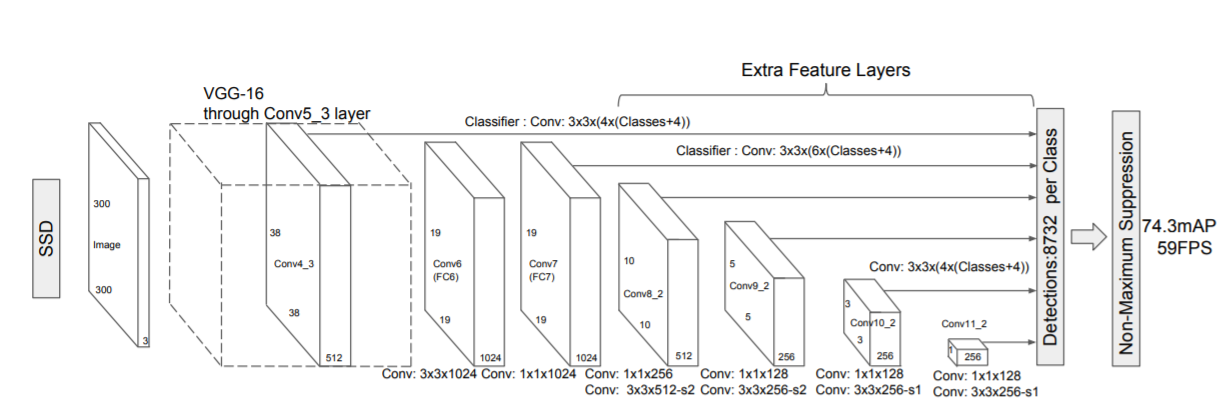
\includegraphics[width=\textwidth]{Sections/2StateOfTheArt/2_images/ssd_arch.png}
        \caption[SSD architecture.]{SSD architecture \cite{Liu2016}.} 
        \label{fig:ssd}
    \end{figure}



    \par The prediction of bounding boxes is done by multiple feature maps of different sizes that represent multiple scales. During prediction time, the network generates scores for the presence of each object category in each default box and produces adjustments to the box to better match the object shape. The network also combines predictions from multiple feature maps with different resolutions to naturally handle objects of various sizes.
    \par SSD is simple relative to methods that require object proposals because it completely eliminates proposal generation and subsequent pixel or feature resampling stages and encapsulates all computation in a single network. This makes SSD easy to train. The core of SSD is predicting category scores and box offsets for a fixed set of default bounding boxes using small convolutional filters applied to feature maps. To achieve high detection accuracy, SSD produces predictions of different scales from feature maps of different scales, and explicitly separate predictions by aspect ratio. These design features lead to simple end-to-end training and high accuracy, even on low resolution input images, further improving the speed vs accuracy trade-off. This approach is based on a feed-forward convolutional network that produces a fixed-size collection of bounding boxes and scores for the presence of object class instances in those boxes, followed by a non-maximum suppression step to produce the final detections \cite{Liu2016}.
   
   

\section{Classification Based Algorithms For Object Detection}
\label{sec:classification}

\par Classification based algorithms work in two stages. Firstly, they select interesting regions from the image and secondly, they classify those regions using convolutional neural networks. The problem with this approach is that it can be extremely slow since a prediction is run for every selected region, however this approach is extremely accurate \cite{Lin2017}. 
\par RCNN, Fast-RCNN and Faster-RCNN are some types of classification based algorithms.  

    \subsection{R-CNN Models Summary}

    \par In the picture below a  compact summary of all of the R-CNN models is illustrated.

    \begin{figure}[H]
        \centering
        \captionsetup{justification=centering}
        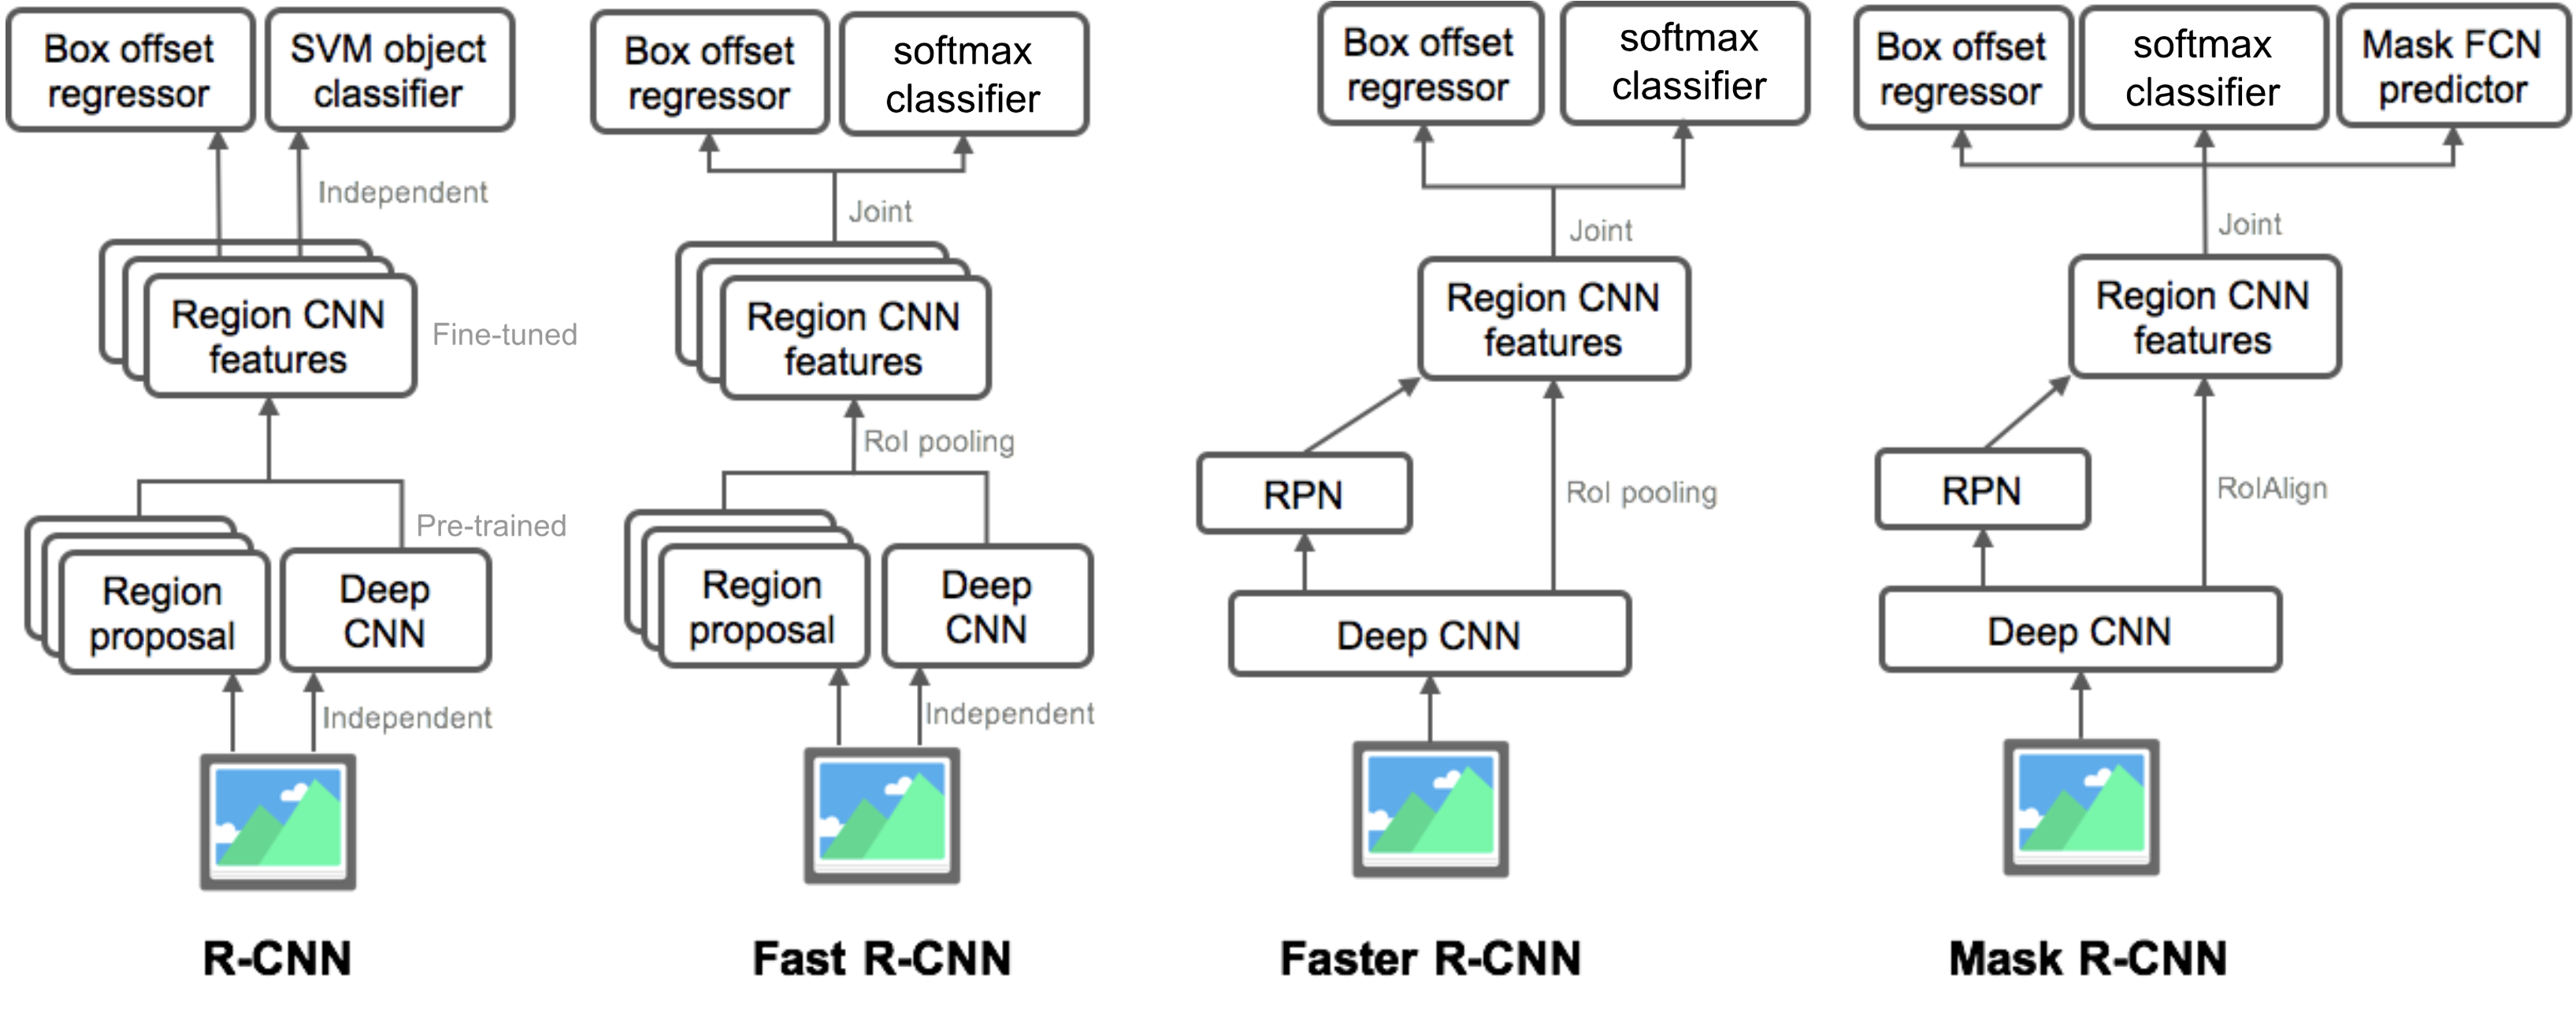
\includegraphics[width=0.65\textwidth]{Sections/2StateOfTheArt/2_images/rcnn-family-summary.png}
        \caption[R-CNN model family summary]{R-CNN model family summary \cite{weng2017detection3}.} 
    \end{figure}

\begin{itemize}
  
    \item\textbf{R-CNN}
\end{itemize}

    
    \par The principal idea behind Region-based Convolutional Networks (R-CNN) can be split into two steps. In the first step the network identifies a number of regions of interest (bounding-box object region candidate) using a selective search method \cite{weng2017detection3}, which is a common algorithm to provide region proposals that can potentially contain objects \cite{weng2017detection1}.
    \par In the second step it extracts CNN features from each region independently for the classification.

    \begin{figure}[H]
        \centering
        \captionsetup{justification=centering}
        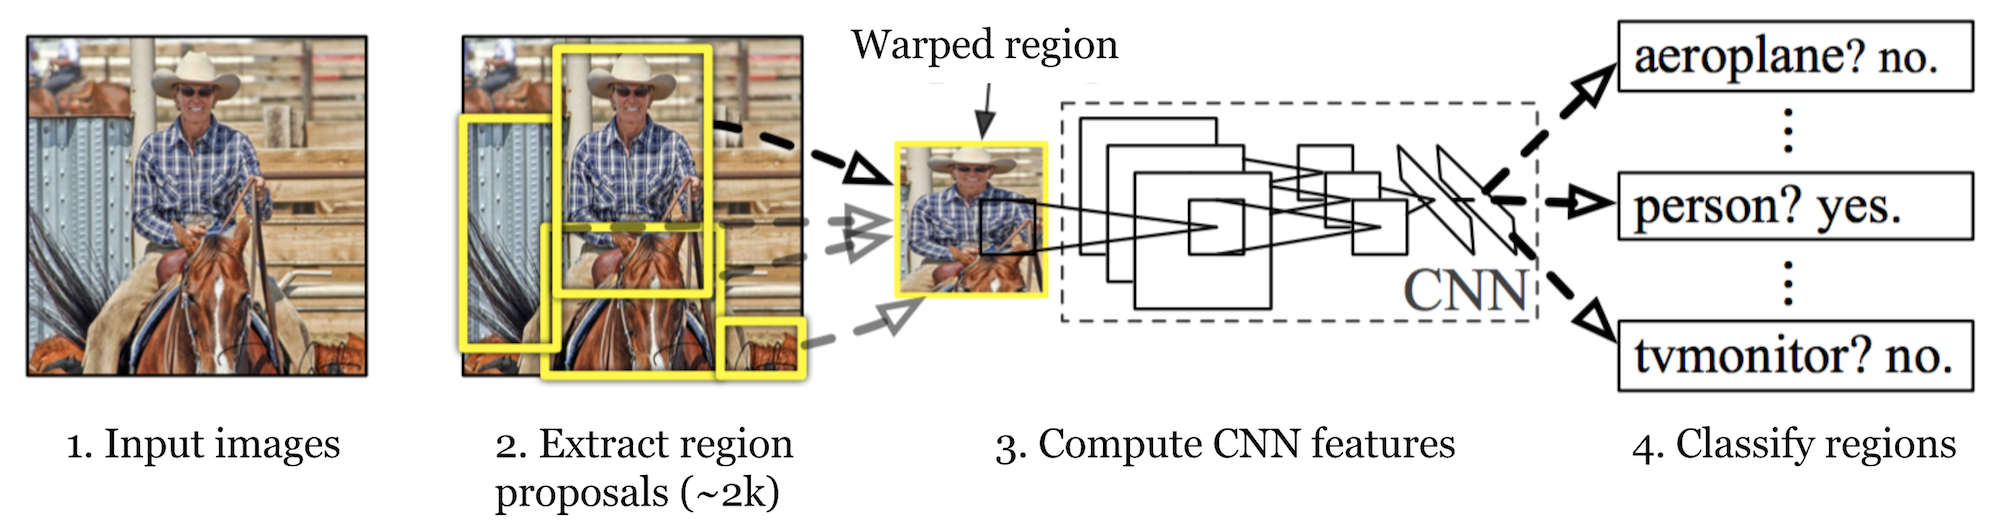
\includegraphics[width=0.75\textwidth]{Sections/2StateOfTheArt/2_images/RCNN.png}
        \caption[R-CNN architecture]{R-CNN architecture \cite{weng2017detection3}.} 
    \end{figure}

    \begin{itemize}
        \item\textbf{Fast R-CNN}
    \end{itemize}
    

    \par The idea behind Fast-RCNN \cite{girshick2015fast} is, as the name implies, to make  R-CNN faster. In order to achieve this, the training procedure was improved by unifying three independent models into one jointly trained framework and increasing shared computation results.
    \par In this new improved network, the CNN feature vectors are not extracted independently for each region proposal, instead this model aggregates them into one CNN forward pass over the entire image and the region proposals share the feature matrix. This feature matrix is then branched to be used for learning the object classifier and the bounding-box regression. In short, computation sharing improves the speed of R-CNN \cite{weng2017detection3}.

    \begin{figure}[H]
        \centering
        \captionsetup{justification=centering}
        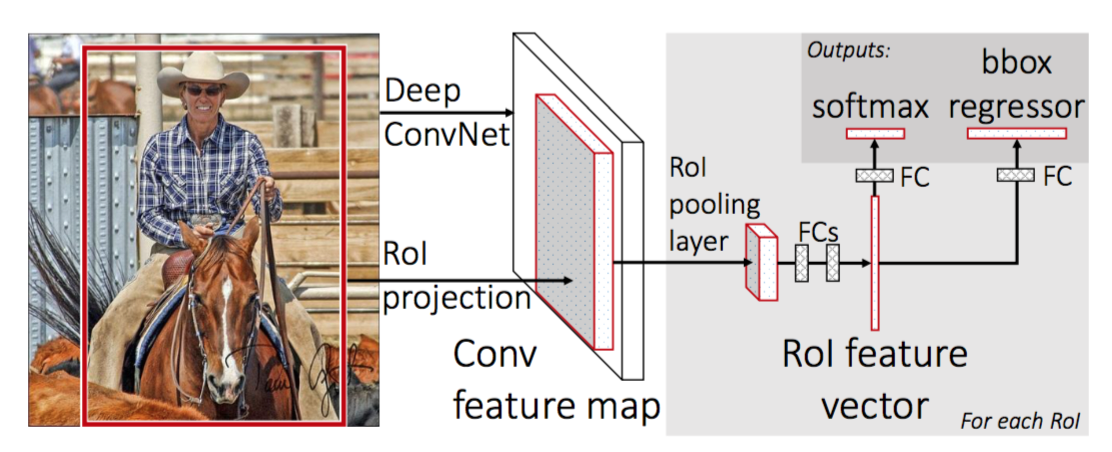
\includegraphics[width=0.55\textwidth]{Sections/2StateOfTheArt/2_images/fast-RCNN.png}
        \caption[Fast R-CNN architecture]{Fast R-CNN architecture \cite{weng2017detection3}.} 
    \end{figure}

    \begin{itemize}
        \item\textbf{Faster R-CNN}
    \end{itemize}
    
    \label{sec:fasterrcnn}

    \par The Faster R-CNN \cite{ren2015faster} improves upon the previous considered solutions since it integrates the region proposal algorithm directly into the CNN model. It can be seen as a single, unified model composed of a region proposal network and fast R-CNN with shared convolutional feature layers \cite{weng2017detection3}.

    \begin{figure}[H]
        \centering
        \captionsetup{justification=centering}
        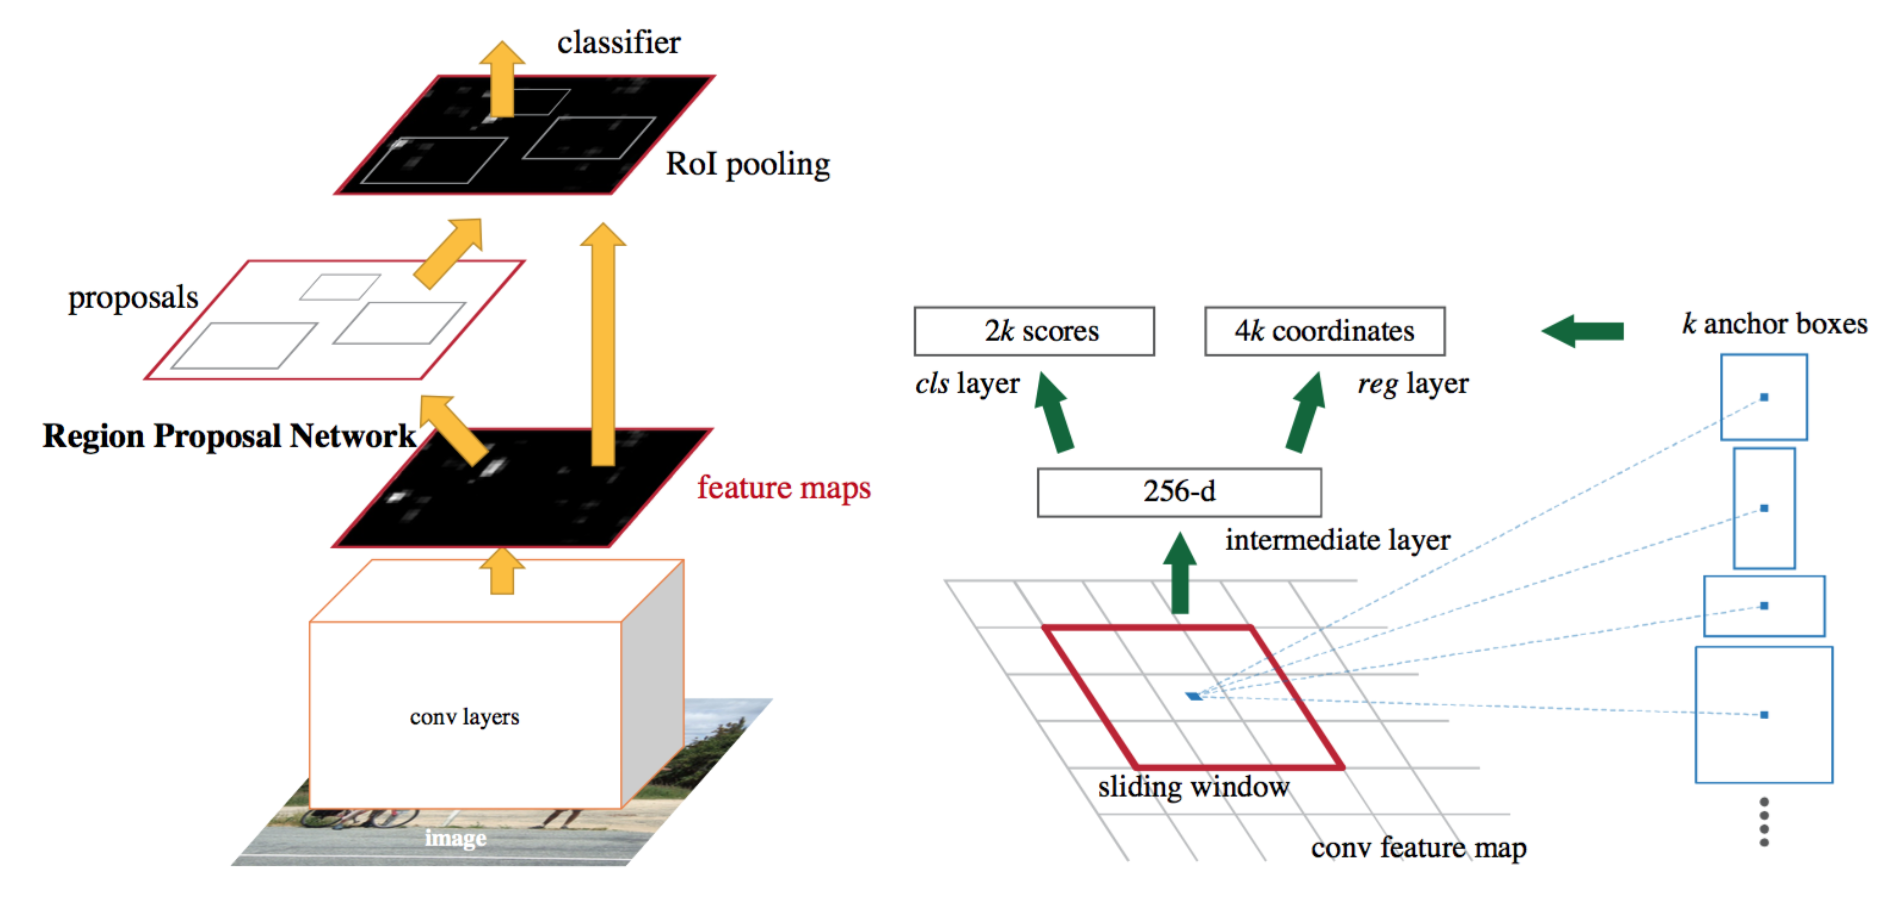
\includegraphics[width=0.5\textwidth]{Sections/2StateOfTheArt/2_images/faster-RCNN.png}
        \caption[Faster R-CNN architecture.]{Faster R-CNN architecture \cite{weng2017detection3}.} 
    \end{figure}
    
    \begin{itemize}
        \item\textbf{Mask R-CNN}
    \end{itemize}
    

    \par The final model of the R-CNN family, Mask R-CNN \cite{he2017mask}, extends faster R-CNN to pixel-level image segmentation by decoupling the classification and the pixel-level mask prediction tasks. It adds a third branch for predicting an object mask in parallel with existing branches for classification and localization, based of the Faster R-CNN framework.This new mask branch predicts a segmentation mask in a pixel-to-pixel manner.
    \par Mask R-CNN improves the region of interest pooling layer because pixel-level segmentation requires much more fine-grained alignment than bounding boxes. This allows the region of interest to more precisely map regions of the original image \cite{weng2017detection3}.

    \begin{figure}[H]
        \centering
        \captionsetup{justification=centering}
        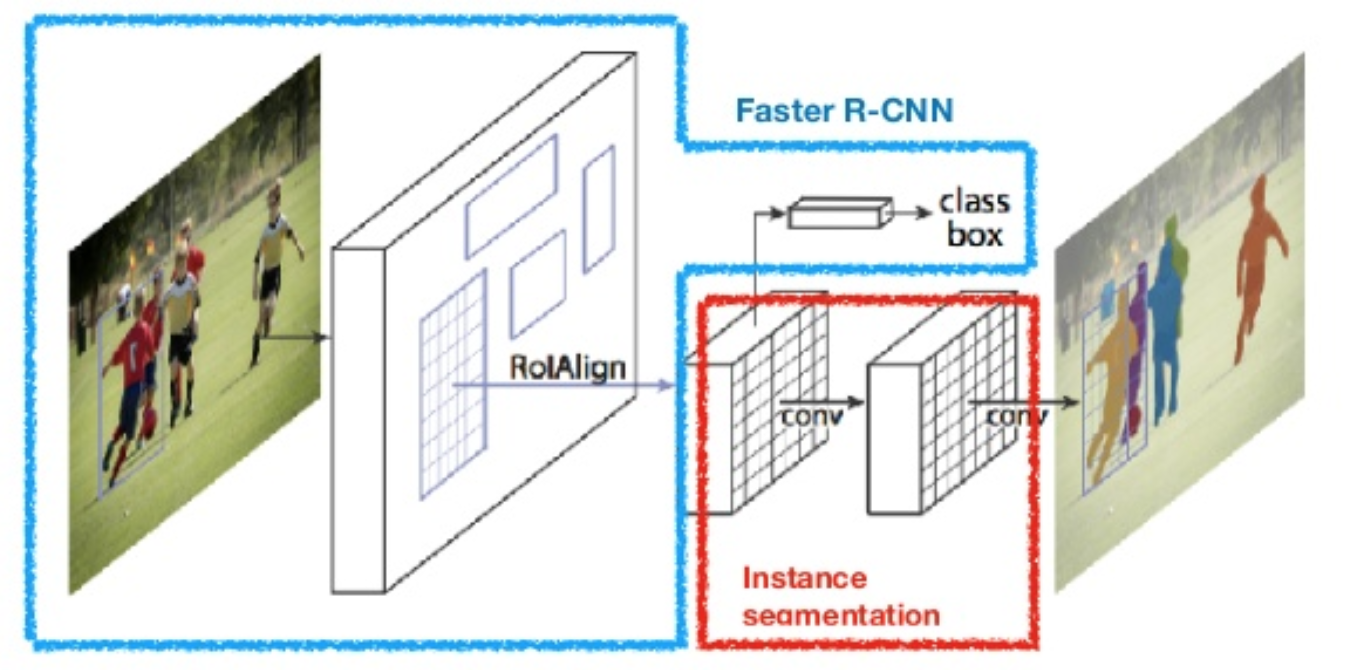
\includegraphics[width=0.5\textwidth]{Sections/2StateOfTheArt/2_images/mask-rcnn.png}
        \caption[Mask R-CNN is a Faster R-CNN model]{Mask R-CNN is a Faster R-CNN model with image segmentation \cite{weng2017detection3}.} 
    \end{figure}

    \newpage  

%%%%%%%%%%%%%%%%%%%%%%%%%%%%%%%%%%%%%%%%%%%%%%%%%%%%%%%%%%%%%%%%%%%%%%%%%%%